\chapter{Results}\label{CH5}
Present the results from following the procedures in \nameref{CH4}, note some observations, but do not discuss them.

\begin{figure}
    \centering
    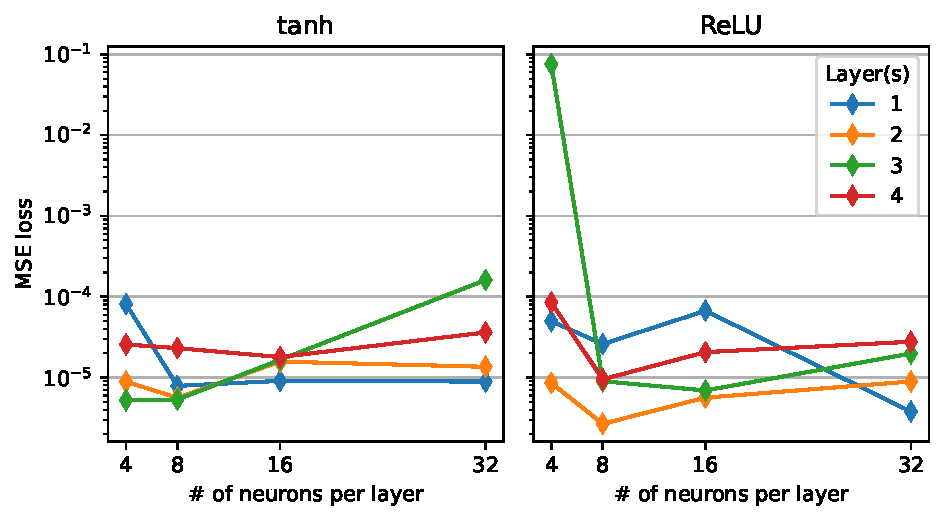
\includegraphics[width=\textwidth]{Chapter/05_results/figures/para1_net.pdf}
    \caption{Final training losses for different network architectures defined by activation function, number of hidden layers and number of neurons per hidden layer}
    \label{fig:para1_net}
\end{figure}

\begin{figure}
    \centering
    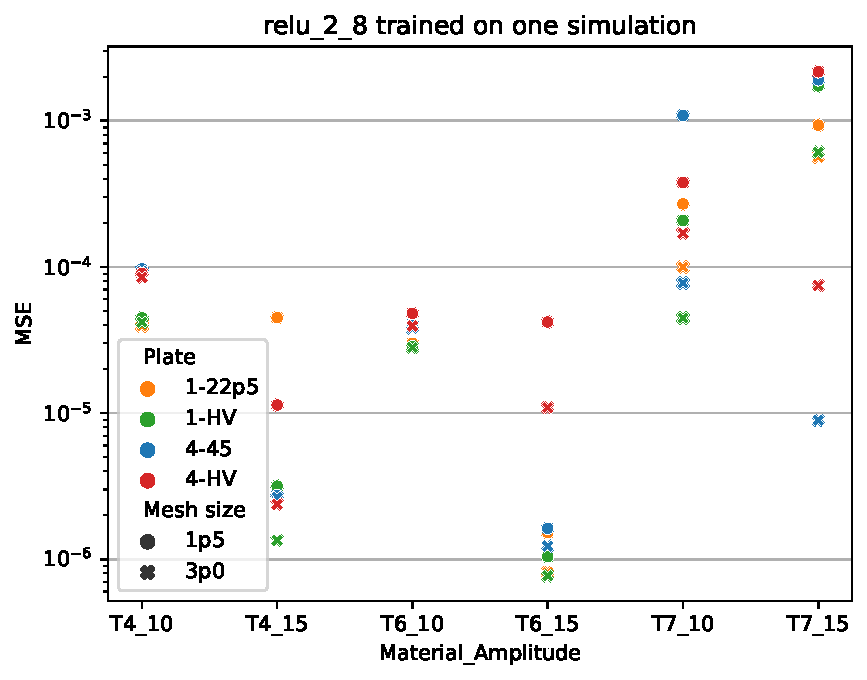
\includegraphics[width=\textwidth]{Chapter/05_results/figures/para1_all.pdf}
    \caption{Bottom text}
    \label{fig:para1_all}
\end{figure}

\begin{figure}
    \centering
    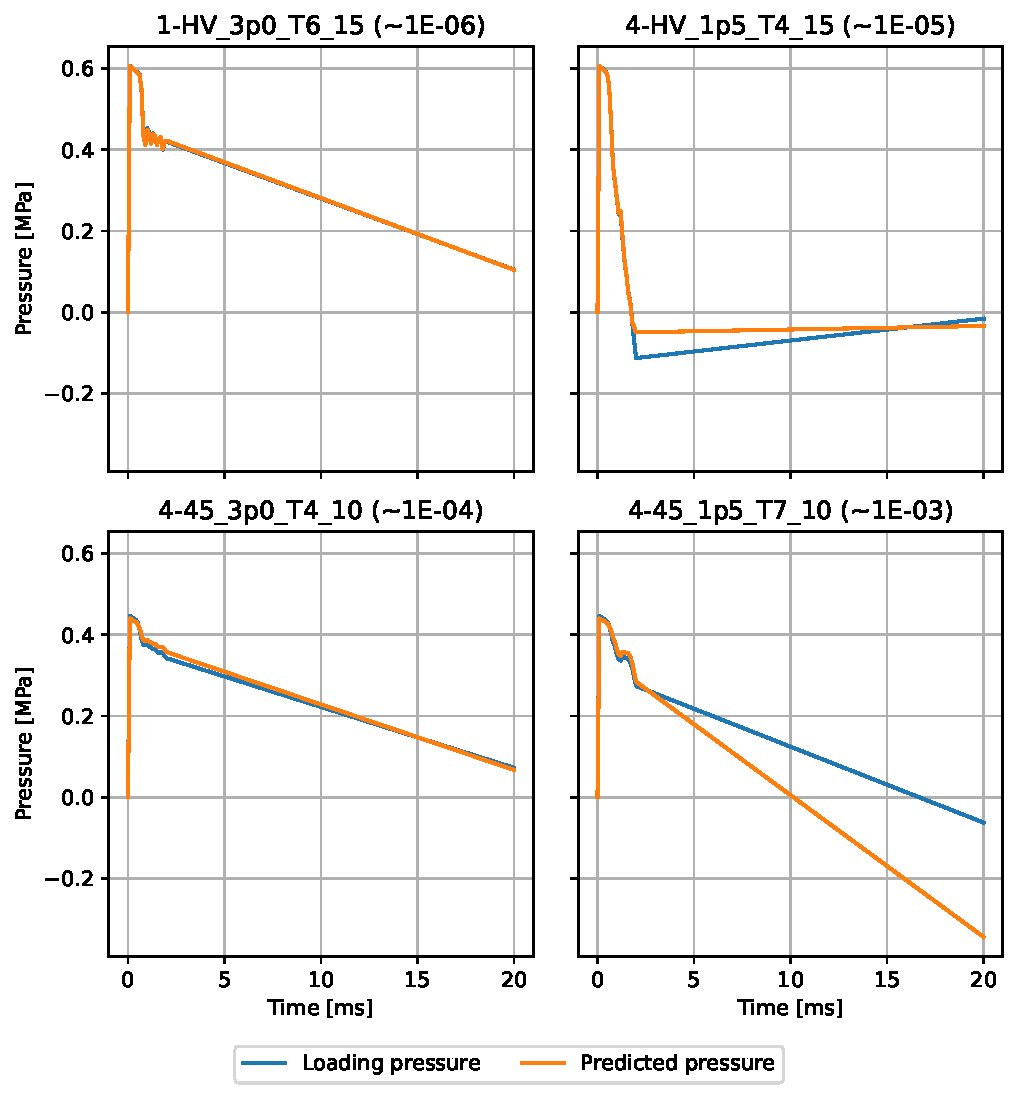
\includegraphics[width=\textwidth]{Chapter/05_results/figures/para1_test.pdf}
    \caption{Bottom text}
    \label{fig:para1_test}
\end{figure}

\begin{figure}
    \centering
    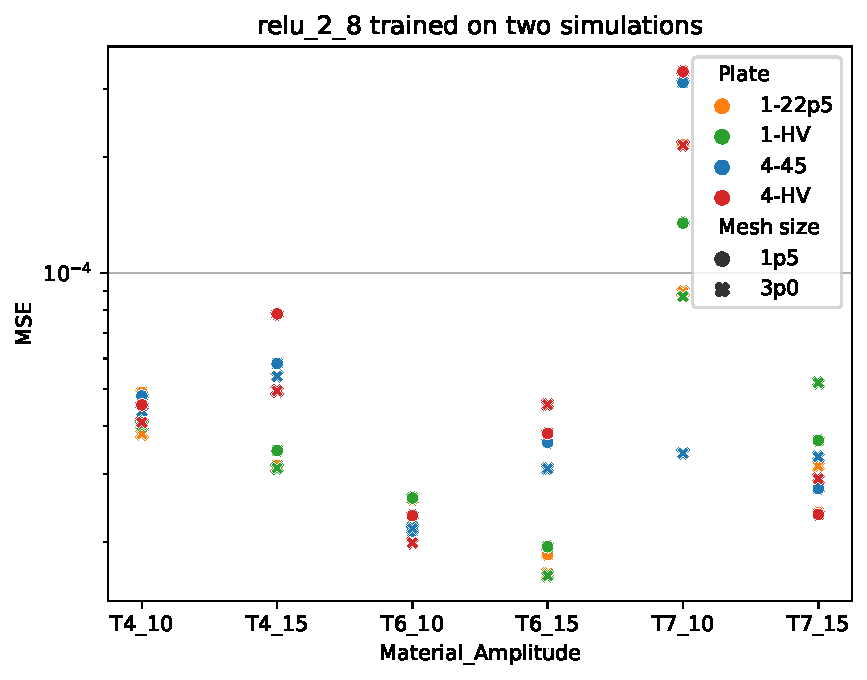
\includegraphics[width=\textwidth]{Chapter/05_results/figures/para2_all.pdf}
    \caption{Bottom text}
    \label{fig:para2_all}
\end{figure}

\begin{figure}
    \centering
    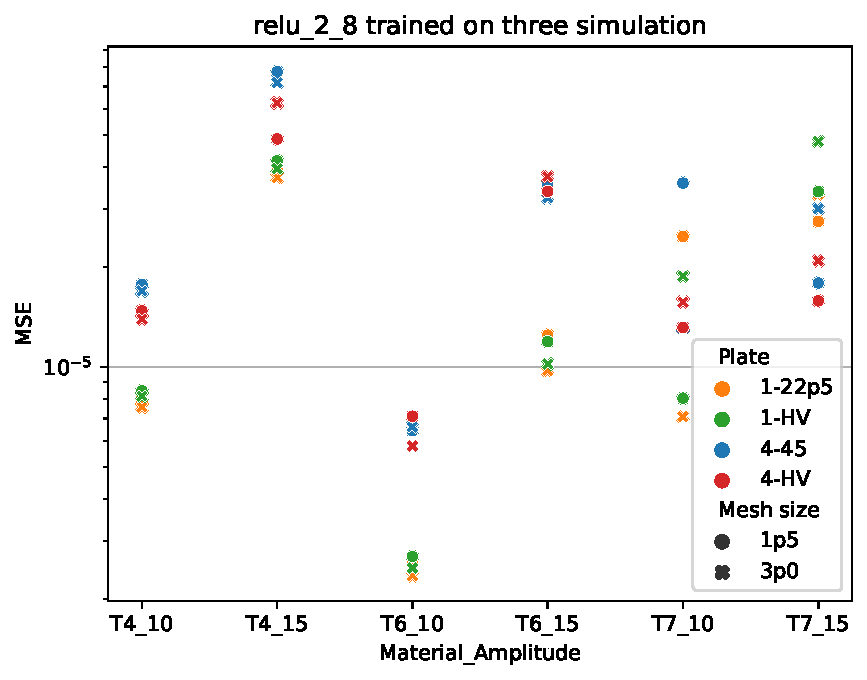
\includegraphics[width=\textwidth]{Chapter/05_results/figures/para3_all.pdf}
    \caption{Bottom text}
    \label{fig:para3_all}
\end{figure}

\begin{figure}
    \centering
    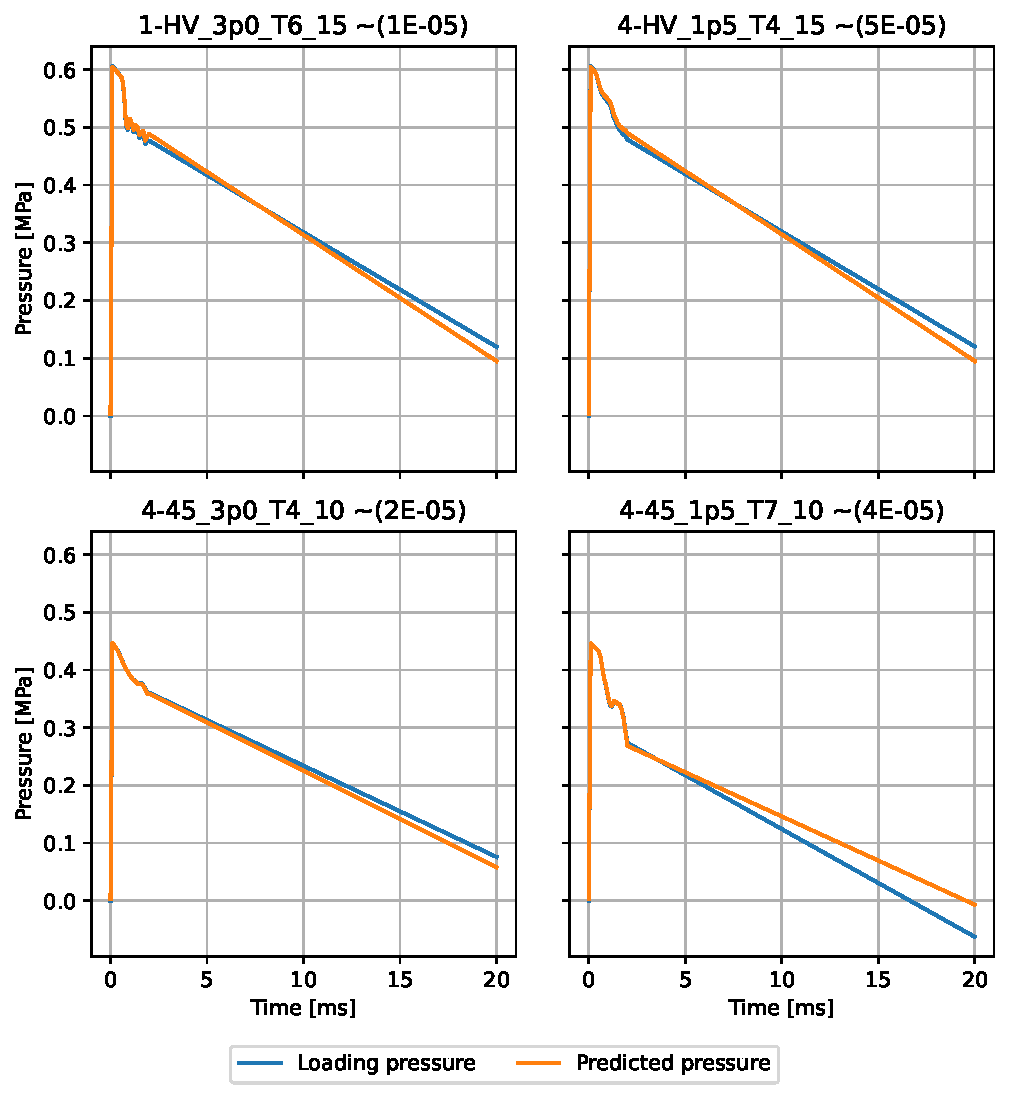
\includegraphics[width=\textwidth]{Chapter/05_results/figures/para3_test.pdf}
    \caption{Bottom text}
    \label{fig:para3_test}
\end{figure}

\begin{figure}
    \centering
    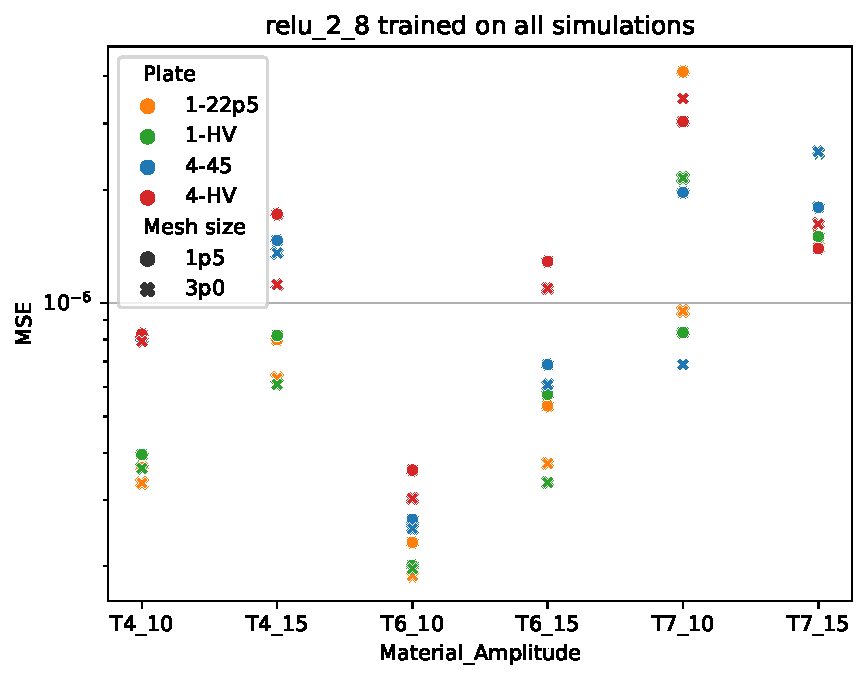
\includegraphics[width=\textwidth]{Chapter/05_results/figures/para4_all.pdf}
    \caption{Bottom text}
    \label{fig:para4_all}
\end{figure}

\begin{figure}
    \centering
    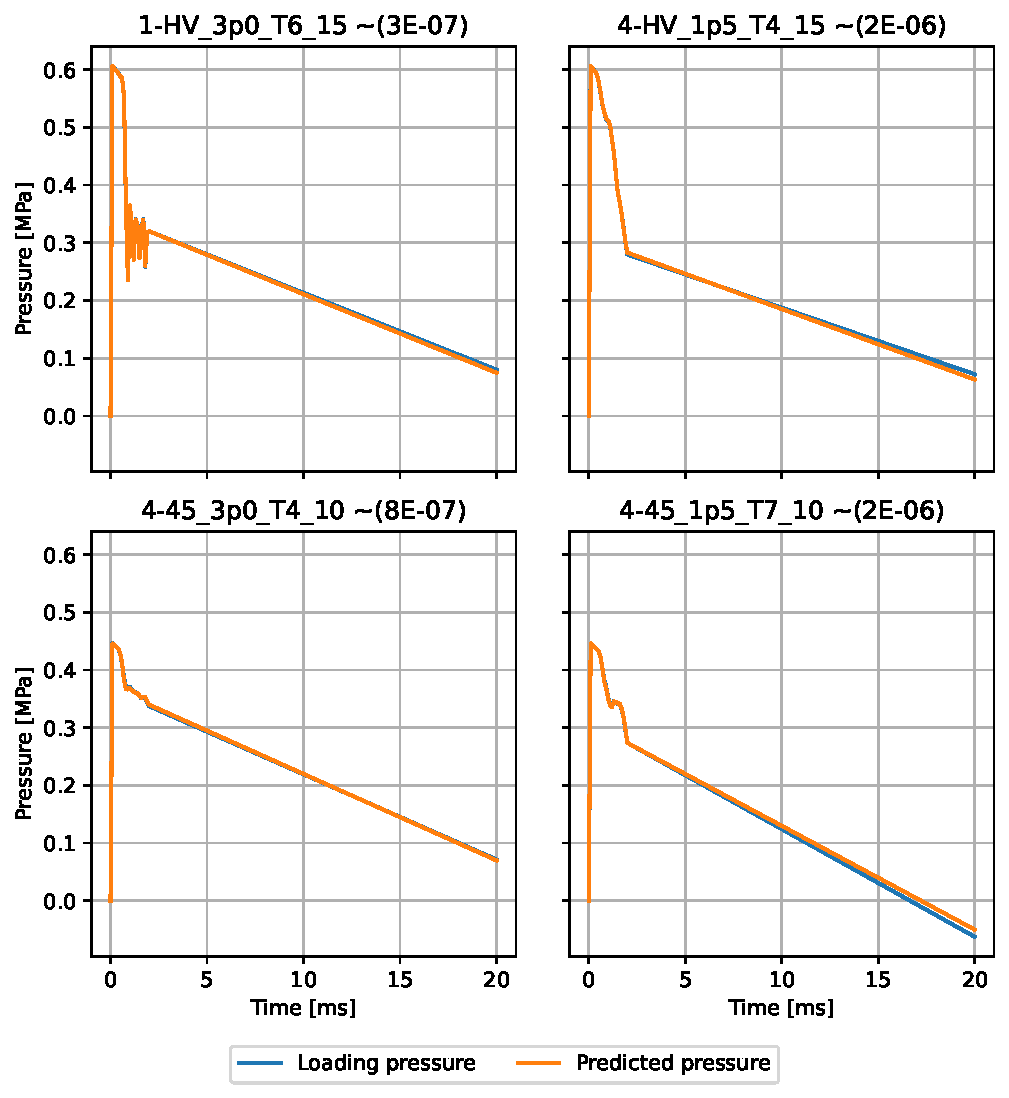
\includegraphics[width=\textwidth]{Chapter/05_results/figures/para4_test.pdf}
    \caption{Bottom text}
    \label{fig:para4_test}
\end{figure}

\begin{figure}
    \centering
    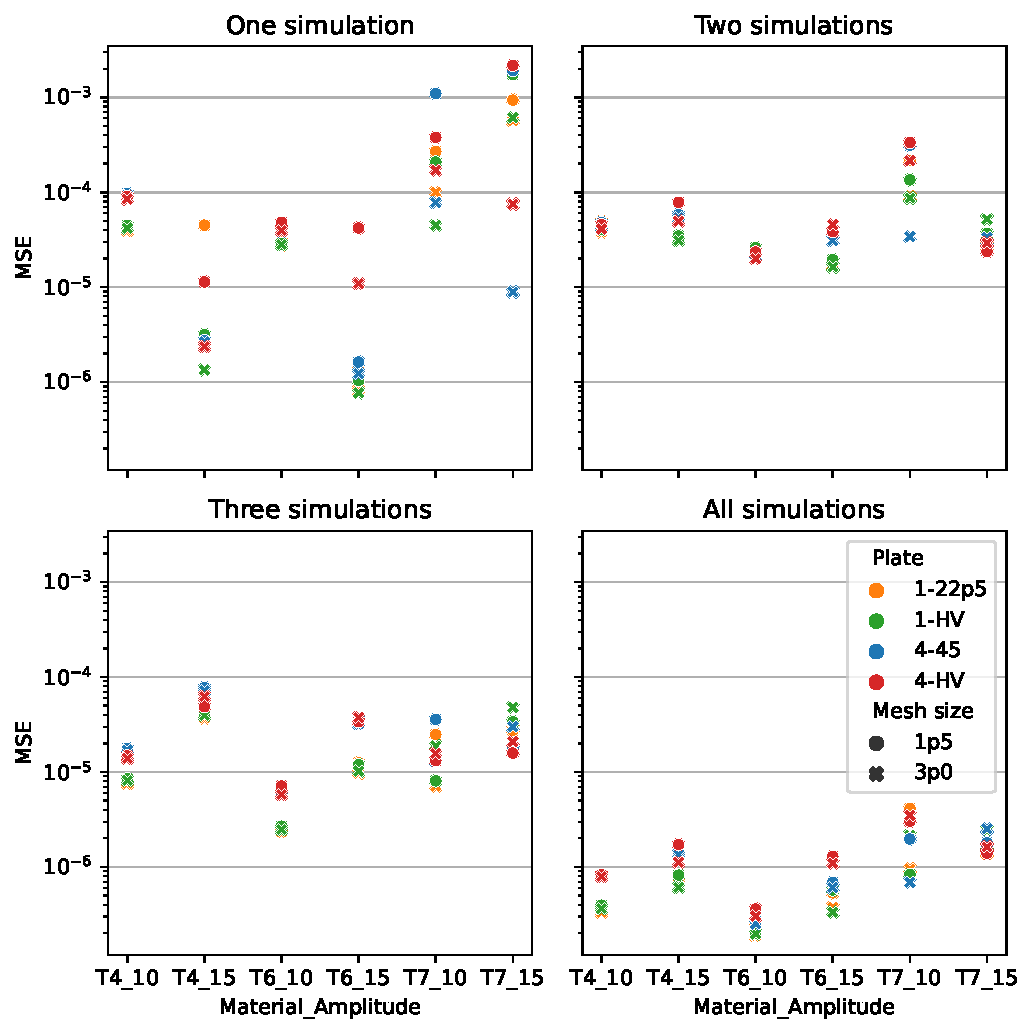
\includegraphics[width=\textwidth]{Chapter/05_results/figures/para_all.pdf}
    \caption{Bottom text}
    \label{fig:para_all}
\end{figure}

\begin{figure}
    \centering
    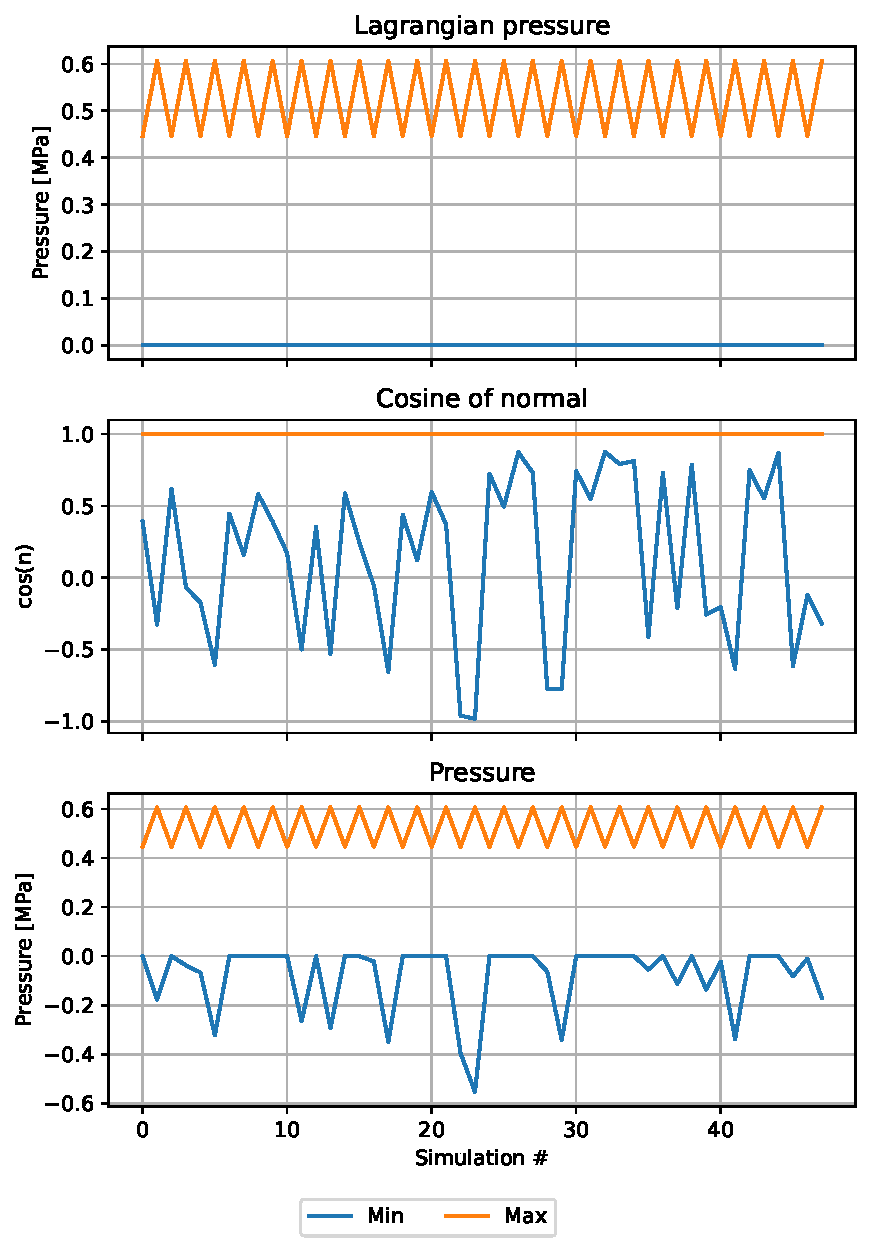
\includegraphics[width=\textwidth]{Chapter/05_results/figures/vars.pdf}
    \caption{Bottom text}
    \label{fig:para_vars}
\end{figure}

\begin{figure}
    \centering
    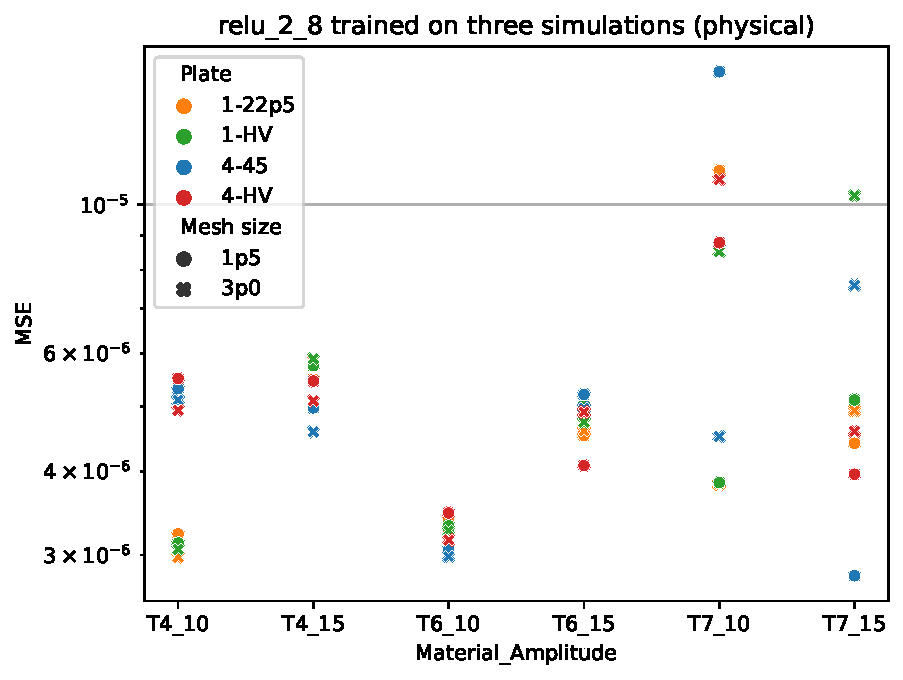
\includegraphics[width=\textwidth]{Chapter/05_results/figures/para5_all.pdf}
    \caption{Bottom text}
    \label{fig:para5_all}
\end{figure}

\begin{figure}
    \centering
    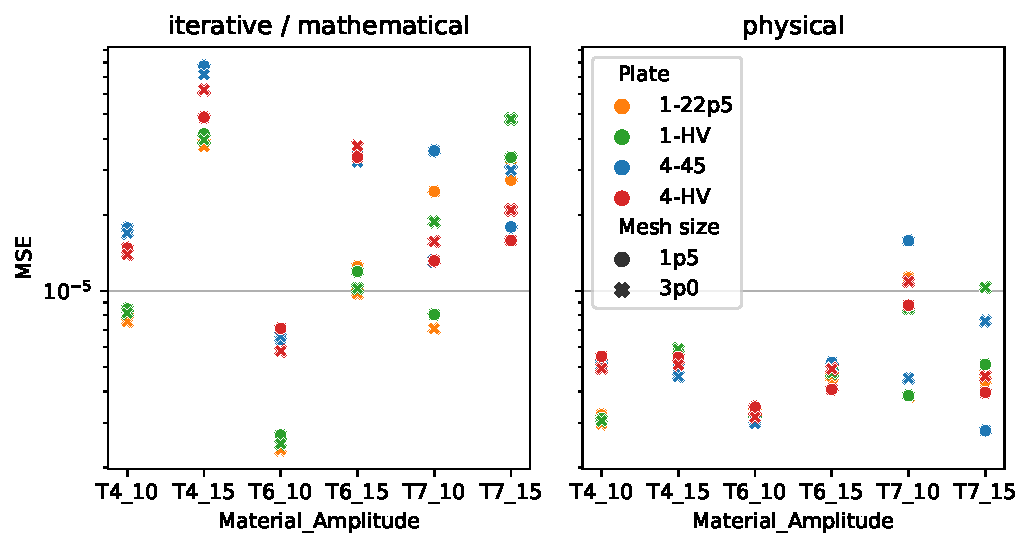
\includegraphics[width=\textwidth]{Chapter/05_results/figures/para3_vs_para5.pdf}
    \caption{Bottom text}
    \label{fig:para3_vs_para5}
\end{figure}